%% Sample file $Id: PBML_article.tex 134 2010-07-01 19:28:04Z popel $
\documentclass{pbml}
%\documentclass[nofonts]{pbml} % for XeLaTeX without Pagella and DejaVu fonts
%\documentclass[color]{pbml} % for color images and hypertext links

% This is a sample file for the PBML article.
% You can compile it with (ordered by preference)
%  1. XeLaTeX with installed fonts TeX Gyre Pagella and DejaVu
%  2. XeLaTeX without the fonts -> you must use \documentclass[nofonts]{pbml}
%  3. pdfLaTeX
%
% In all three methods, you can use Unicode (utf8) encoding for special letters
% (so instead of na\"{i}ve you can write directly naïve).
% Note that with methods 2 and 3, your output will be slightly DIFFERENT than
% our final print version (different line breaks and page breaks).
% See the end of this file for more information.

% Packages
% ========
% In this place you can load required packages by the \usepackage commands.
% The following packages are loaded automatically by the class:
% euler    (for math fonts)
% graphicx (for inclusion of images)
% multicol (for multicolumn typesetting)
% natbib   (for bibliography citations)
% amssymb  (for various symbols)
% If XeLaTeX is used, fontspec and xltxtra are loaded as well.

% Definitions
% ===========
% You can use your own macros defined by \newcommand, \providecommand,
% \DeclareRobustCommand (or even by \def) as well as environments declared by
% \newenvironment. You can also use \newcounter in order to declare your own counters.

\begin{document}

% Document title and authors
% ==========================
% Due to journal organization, the article title and authors must be specified
% AFTER \begin{document}. Note that \subtitle is not allowed anymore due to
% problems with indexing in science databases. If needed use colon in the title.

\title{Title of My Article\titlelinebreak{} with a Forced Linebreak}


% Now put the affiliated institutes first, then author names and the labels
% of their institutes in the "institute" field. The order of institutes and
% authors printed below the title will be the same as the order of your commands.
% Each author can be associated with more than one institute.
% One author must be chosen as the "corresponding author" (using attribute
% corresponding) and his or her email and full address must be provided.
% PLEASE, use Unicode (utf8) encoding (e.g ï instead of \"{i}).

\institute{label1}{IBM}
\institute{label2}{CNGL, Dublin City University}
\institute{label3}{Center for Language and Speech Processing, Johns Hopkins University}
\institute{label4}{Carnegie Mellon University}

\author{
  firstname=Humpty,
  surname=Dumpty,
  institute=label1,
}
\author{
  firstname=Mock,
  surname=Turtle,
  institute={label2,label4},
  corresponding=yes,
  email={turtle@seacoast.wl},
  address={Carnegie Mellon University\\407 S. Craig Street, Pittsburgh, PA 15213, United States}
}
\author{
  firstname=Cheshire,
  initials=C.,
  surname=Cat,
  institute=label3,
}

% If all authors belong to the same institute, you can use simpler syntax:
% \institute{}{Charles University in Prague, Faculty of Mathematics and Physics, Institute of Formal and Applied Linguistics}
% \author{firstname=Humpty, surname=Dumpty}
% \author{firstname=Mock, surname=Turtle,
%   corresponding=yes,
%   email={turtle@seacoast.wl},
%   address={Institute of Formal and Applied Linguistics\\
%            Faculty of Mathematics and Physics,\\
%            Charles University in Prague\\
%            Malostranské náměstí 25\\
%            118 00 Praha 1, Czech Republic}}
% \author{firstname=Cheshire, surname=Cat}


% The title and authors' names are used in the running head. If they are
% long, you should define short versions. These definitions are optional. You
% define them only if they are needed. The example follows:
\shorttitle{Short title}
\shortauthor{H. Dumpty, M. Turtle, C. Cat}

% Now print the title by:
\PBMLmaketitle


% Abstract
% ========
% The abstract is placed within the "abstract" environment. It is a mandatory
% part of the article. PLEASE, do not use your own macros in abstract, if possible.

\begin{abstract}
The abstract of the article...
\end{abstract}

\section{Introduction}
% The body of the article
% =======================
% The PBML class is modelled after the standard article class. This means
% that you can use almost everything that is allowed in articles as described
% in the textbooks of LaTeX. We support sectioning commands \section,
% \subsection and \subsubsection.

% In addition to the \cite command, you can use natbib style of citations.
% PLEASE, use \citet instead of \cite if the author names are part of the sentence.
\citet{PDT2} show \ldots \\ % This renders as "Hajič et al. (2006) show" instead of "(Hajič et al., 2006) show".
\ldots tree-based annotation (e.g.~\citealp{PDT2}).


% For figures and tables always use "figure" resp. "table" floating environments
% and always supply a caption. See the paragraph about color images below.
\begin{figure}
 \begin{center}
  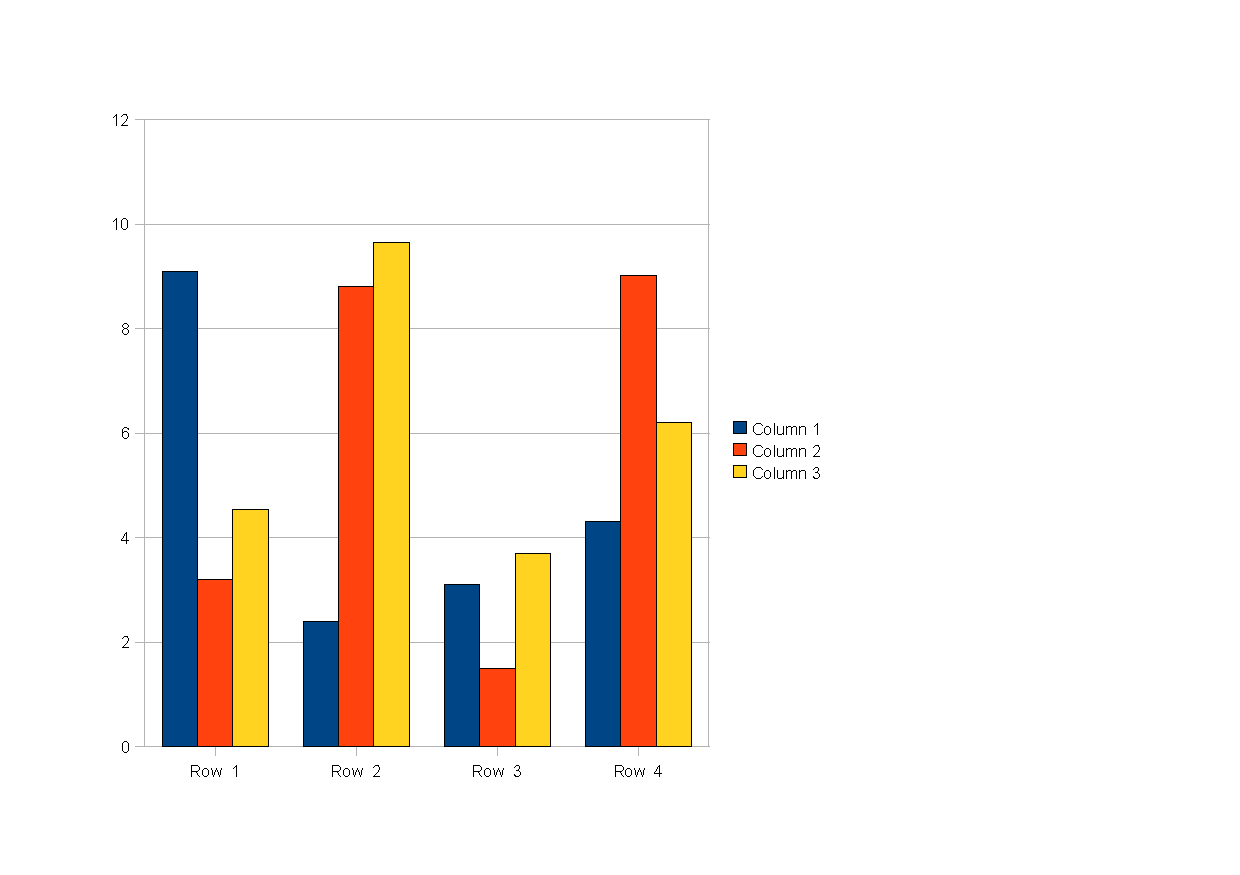
\includegraphics[width=\textwidth]{example_figure}
  \caption{Example figure}\label{fig:example}
 \end{center}
\end{figure}

\section*{Acknowledgements}
This research is supported by \ldots

% Bibliography
% ============
% You may either enter the bibliography manually, possibly making use of
% \label and \ref, or use BibTeX. The bibliography style is set
% automatically. You process the bibliography by BibTeX in the
% standard way and include it by:
\bibliography{mybib}

% If needed, add appendices here
%\section*{Appendix A: \ldots}

\correspondingaddress
\end{document}

% ======= Additional information ==========

% XeLaTeX
% =======
% The Prague Bulletin of Mathematical Linguistics is typeset by XeLaTeX.
% It is not required that you use XeLaTeX and the same fonts as will be used in the
% journal but it is better to do so if you could (so you have the same line and page breaks).
% If XeLaTeX is not available on your computer, you can even used standard LaTeX.

% Fonts
% =====
% In the printed version, fonts TeX Gyre Pagella (shipped with TeX Live 2008 or later)
% and DejaVu (http://dejavu.sourceforge.net/wiki/index.php/Main_Page)
% will be used. If you have XeLaTeX but not these fonts, you may need to install
% the fonts somewhere where your system (fontconfig) can find them. On Linux,
% try something like this:
% ln -s YOUR-TEXLIVE/2008/texmf-dist/fonts/opentype/public/ \
%  ${HOME}/.fonts/texlive-2008-otf-public
% If you are not able to install these fonts, you can instruct XeLaTeX
% to use its default fonts by \document[nofonts]{pbml}.

% If you want to typset examples in east Asian scripts, you have to use
% OpenType Unicode fonts that are freely redistributable and you have to
% include them with your article. If you must use nonfree or non-Unicode
% fonts, you must supply the examples as EPS or PDF with fonts embedded in
% the files (as the required subset).
% If encountering problems with the "bidi" package, contact pbml@ufal.mff.cuni.cz.

% Vector Graphics
% ===============
% The most portable graphics package is tikz which is a front end to pgf.
% This package is fully supported both in standard LaTeX and XeLaTeX.
% PSTricks is not currently available for XeLaTeX.

% Color Images
% ============
% The printed version of PBML does not allow color figures, so please convert
% all your figures to grayscale (or black&white), make sure they are legible
% and put them in a subdirectory called "grayscale".
% When specifying the filename in \includegraphics DO NOT include the
% subdirectory.
% Optionally, in addition to the default grayscale images, you can add also
% color versions of the figures to be published in the online version.
% Put such images in a subdirectory called "color" with the same filenames
% as the grayscale ones.
% To temporarily switch to color output and hypertext links, use
% \documentclass[color]{pbml}

% Including images and other files
% ===================================
% When loading the file you must use a relative path, never the full path.
% Load the images by \includegraphics
% and other files by \input, never use \include.
